\section{Effektivitet af cuts}
\begin{frame}{Effekten af cuts}
	Hvordan ser usorteret data ud?\\
	\begin{figure}
		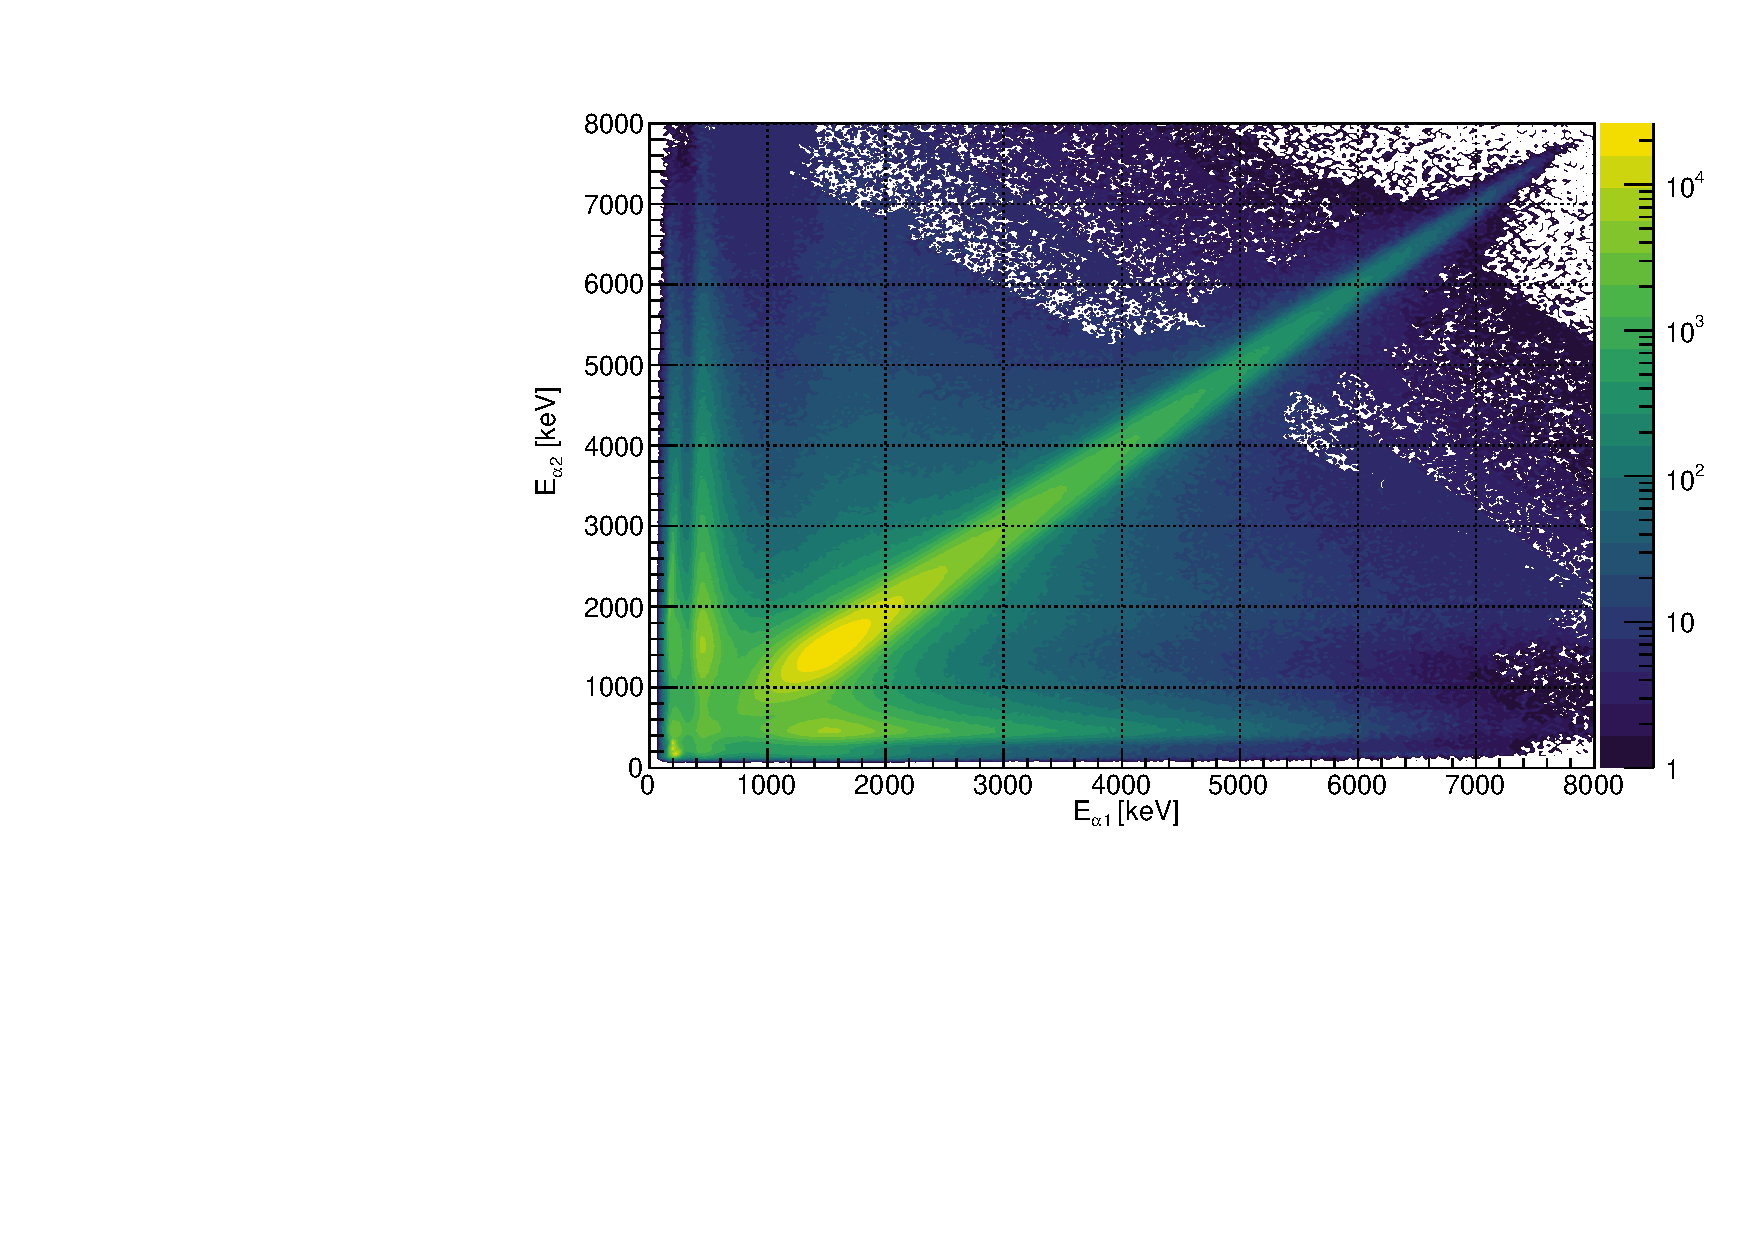
\includegraphics[width=0.7\columnwidth]{../figures/EENoCuts.pdf}
	\end{figure}
\end{frame}

\begin{frame}{Effekten af vinkel cut}
	Indbyrdes vinkel på maksimalt $161\degree$\\
	\begin{figure}
		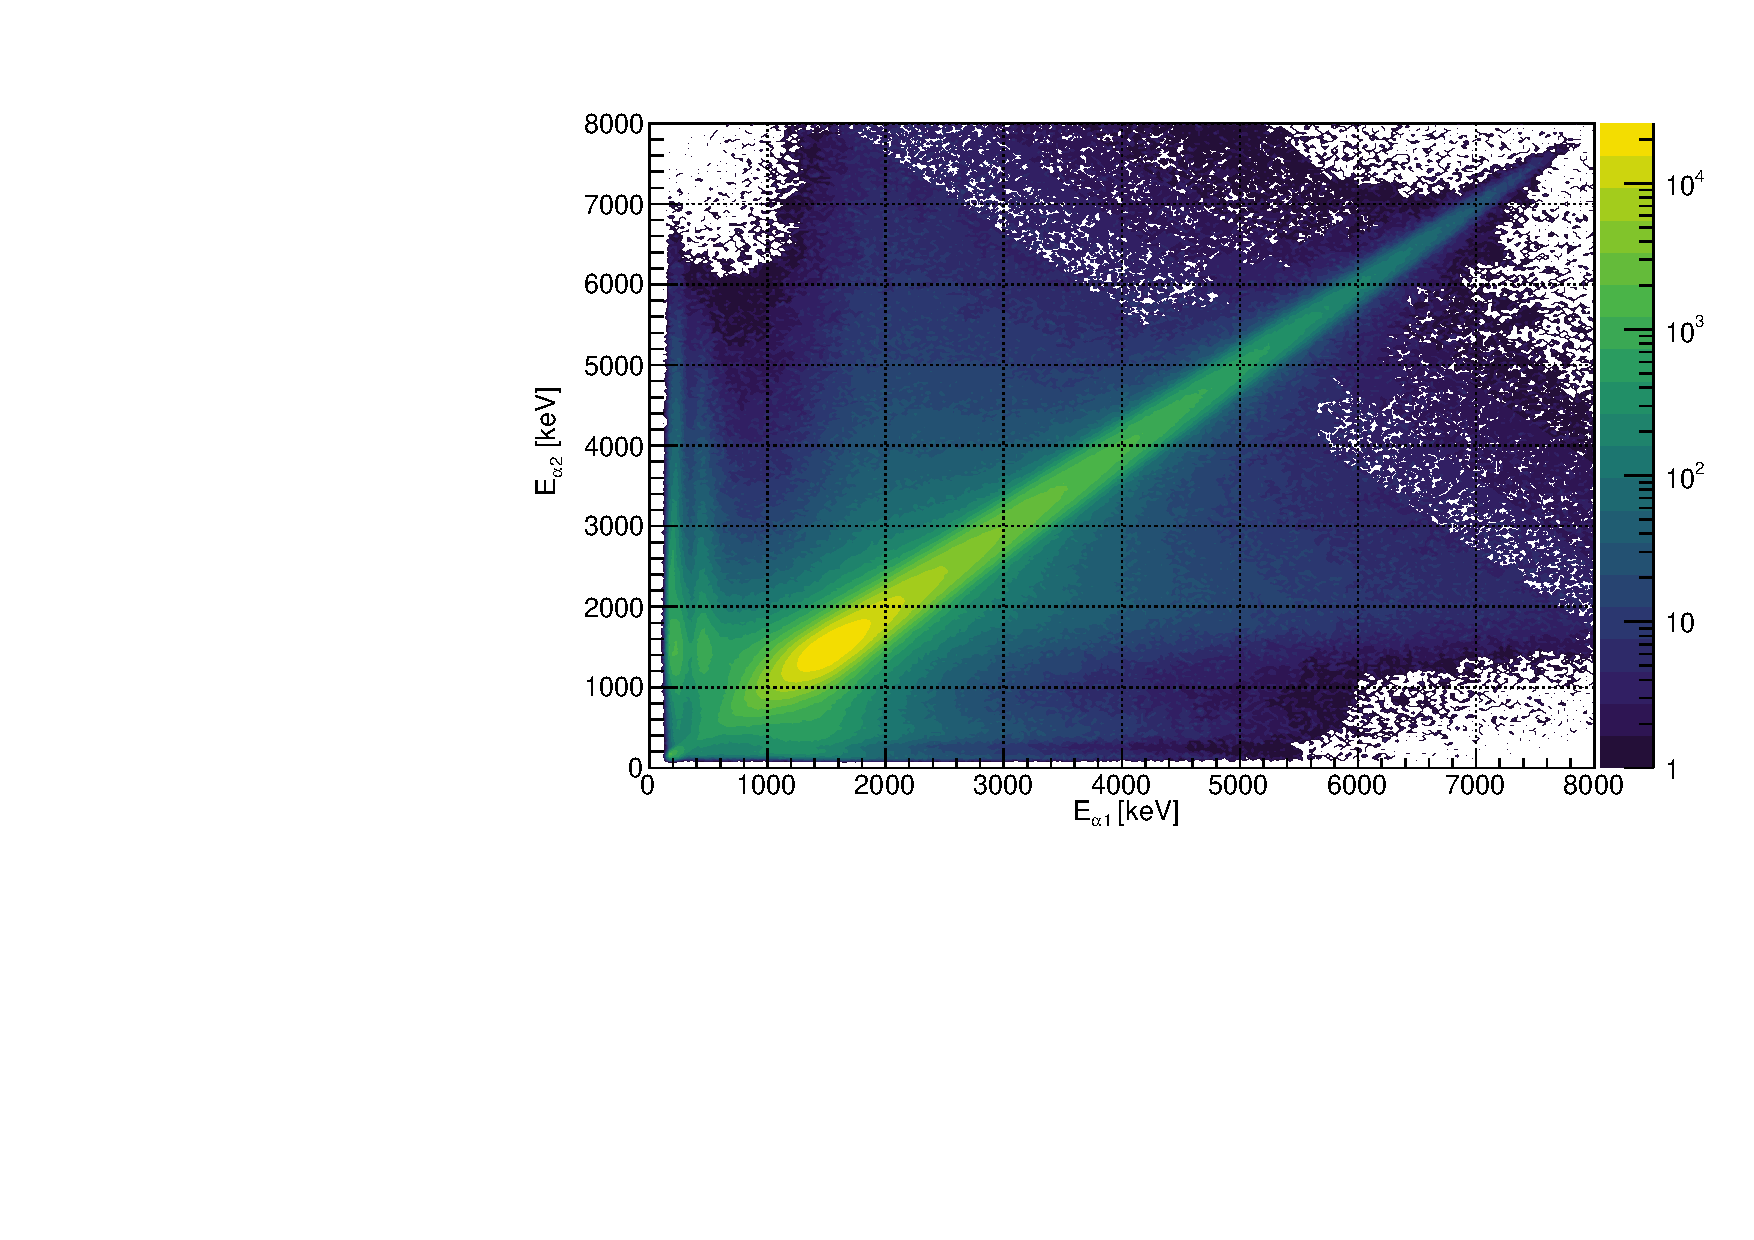
\includegraphics[width=0.7\columnwidth]{../figures/EEAngleCut.pdf}
	\end{figure}
\end{frame}

\begin{frame}{Effekten af impuls cut}
	Total impuls på maksimalt \SI{40}{MeV/c}
	\begin{figure}
		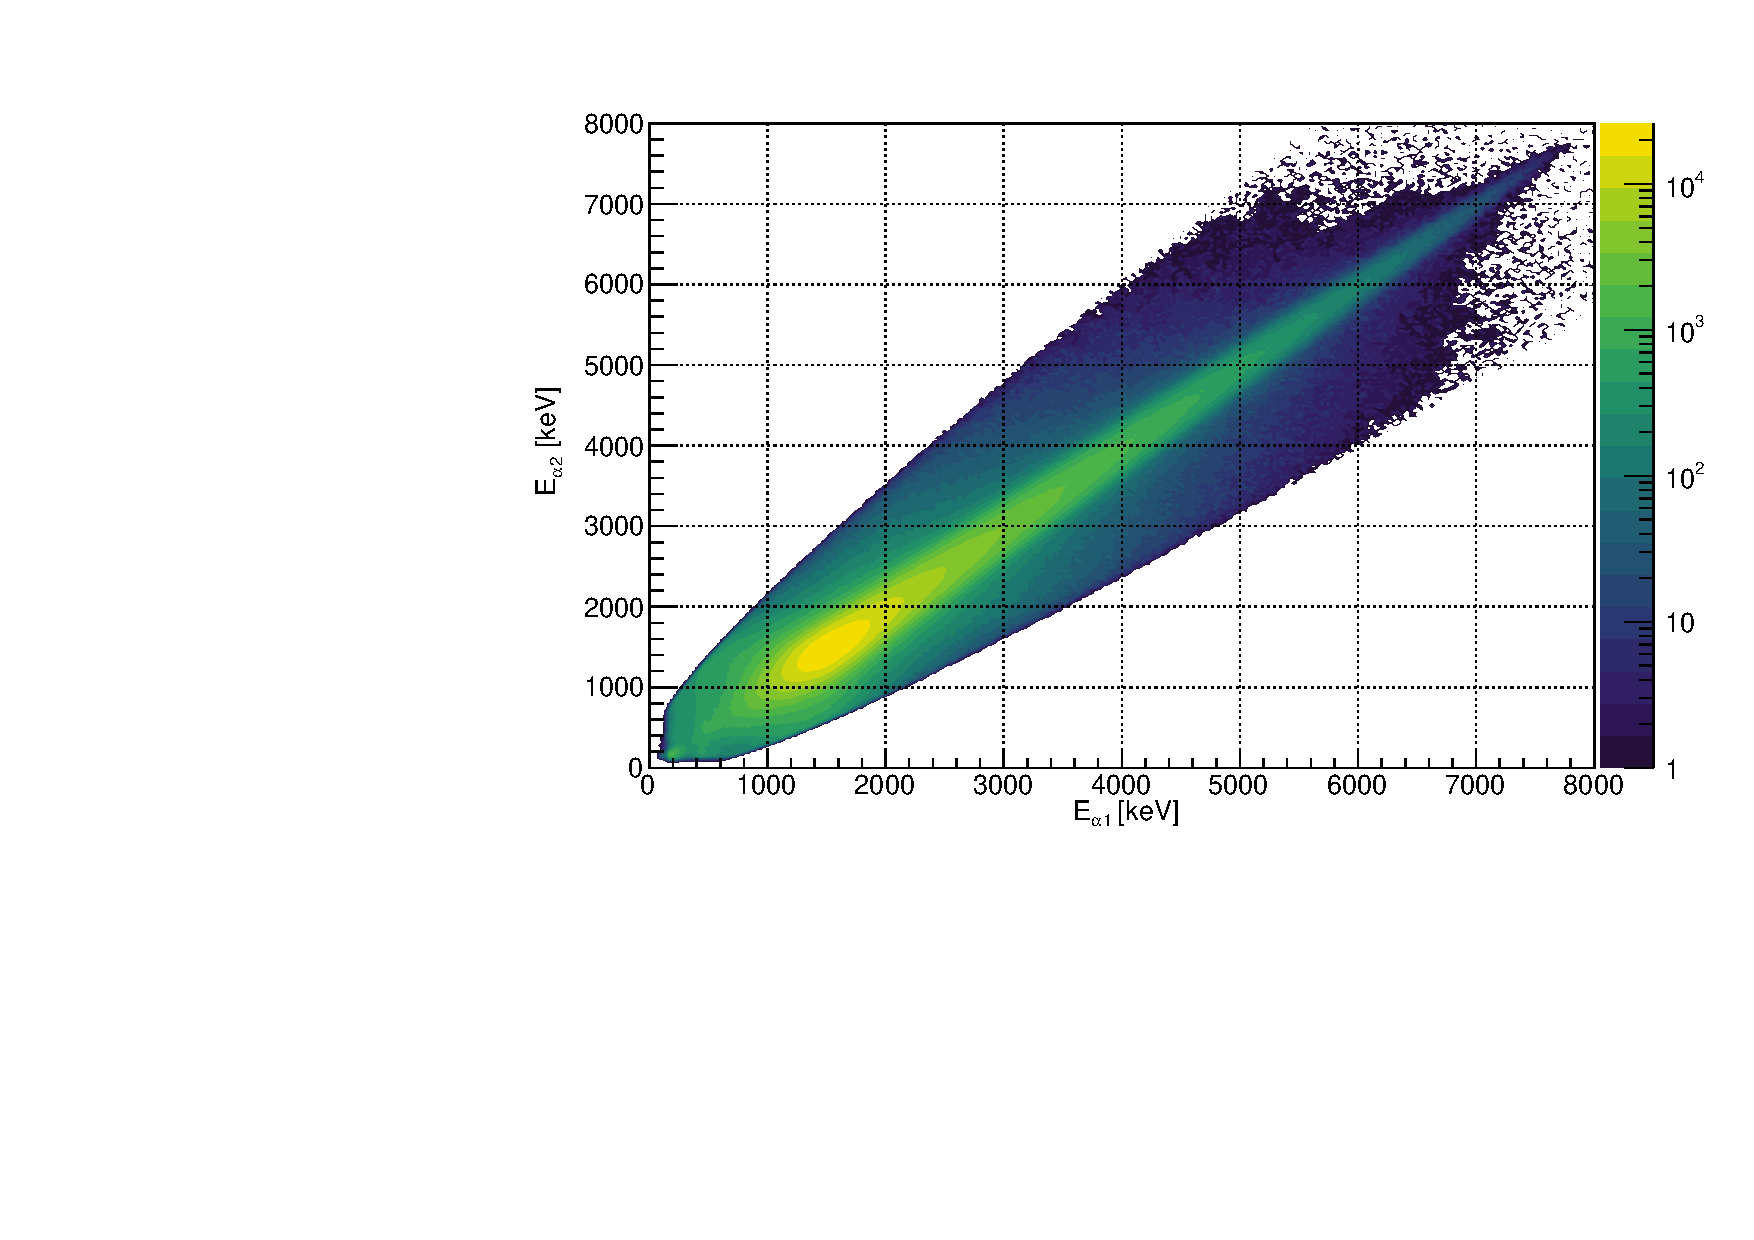
\includegraphics[width=.7\columnwidth]{../figures/EEMomentumCut.pdf}
	\end{figure}
\end{frame}

\begin{frame}{Effekten af \be-multiplicitet cut}
	Minimum 1 \be-partikel i et event
	\begin{figure}
		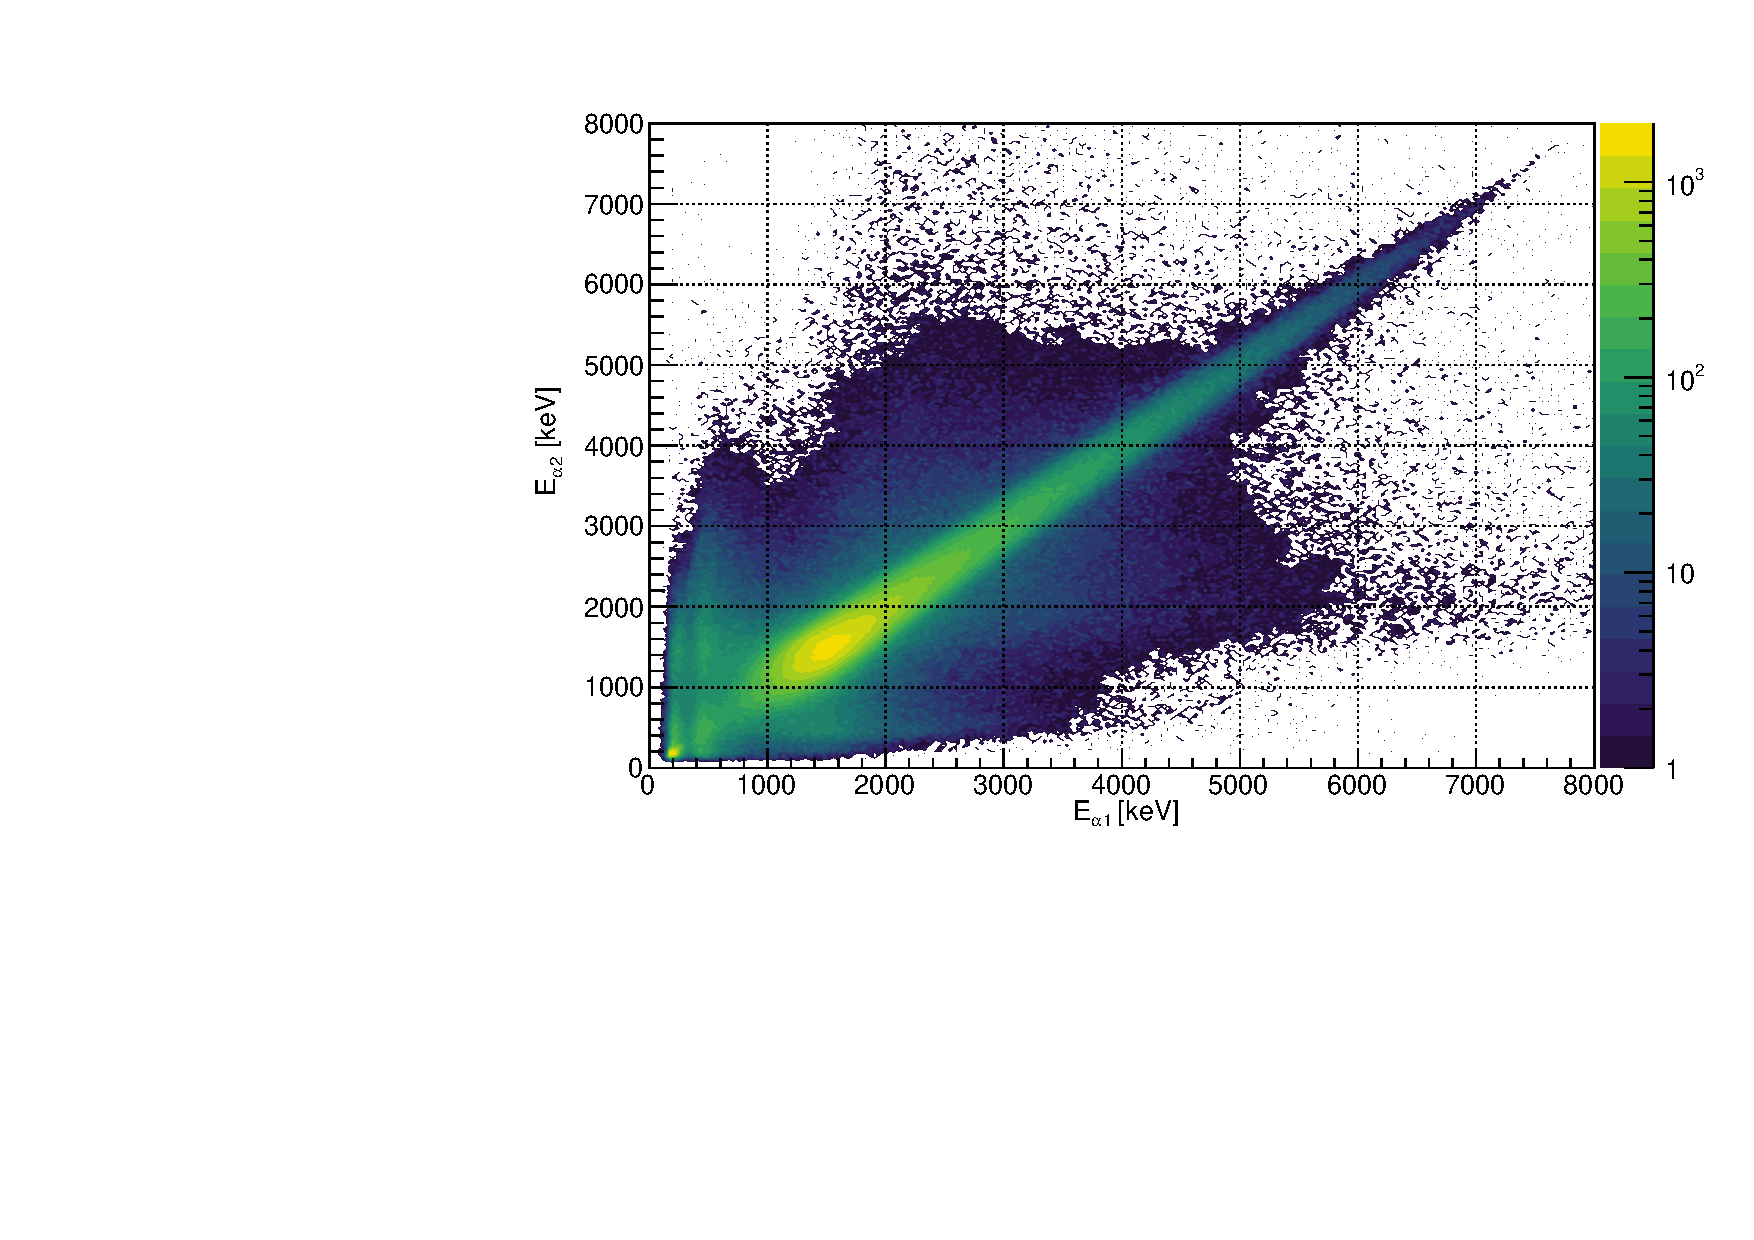
\includegraphics[width=.7\columnwidth]{../figures/EEBetaMulCut.pdf}
	\end{figure}
\end{frame}

\begin{frame}{Effekten af alle cuts}
	Alle cuts 
	\begin{figure}
		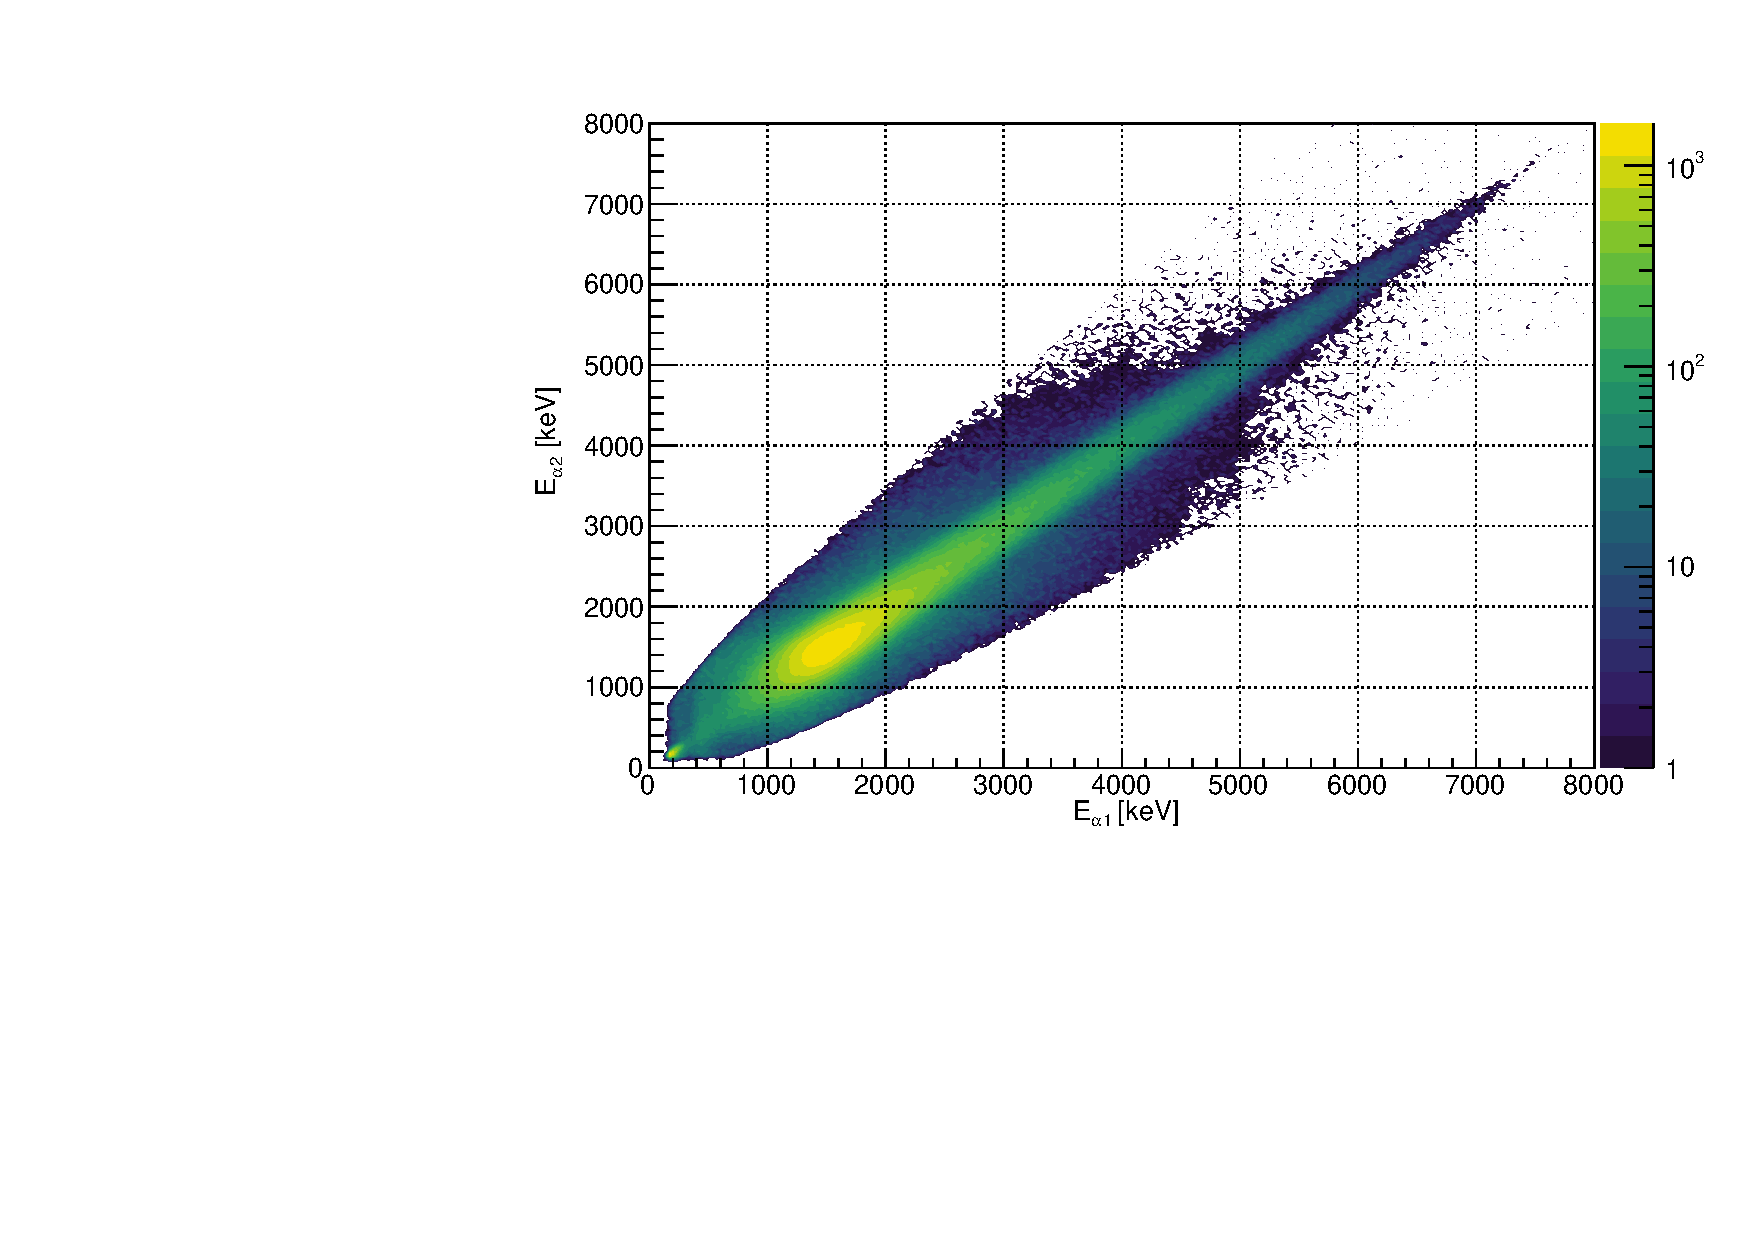
\includegraphics[width=.7\columnwidth]{../figures/EE.pdf}
	\end{figure}
\end{frame}

\begin{frame}{Cut sammenligning}
	Energi spektrum for enkelt \al-partikel
	\begin{figure}
		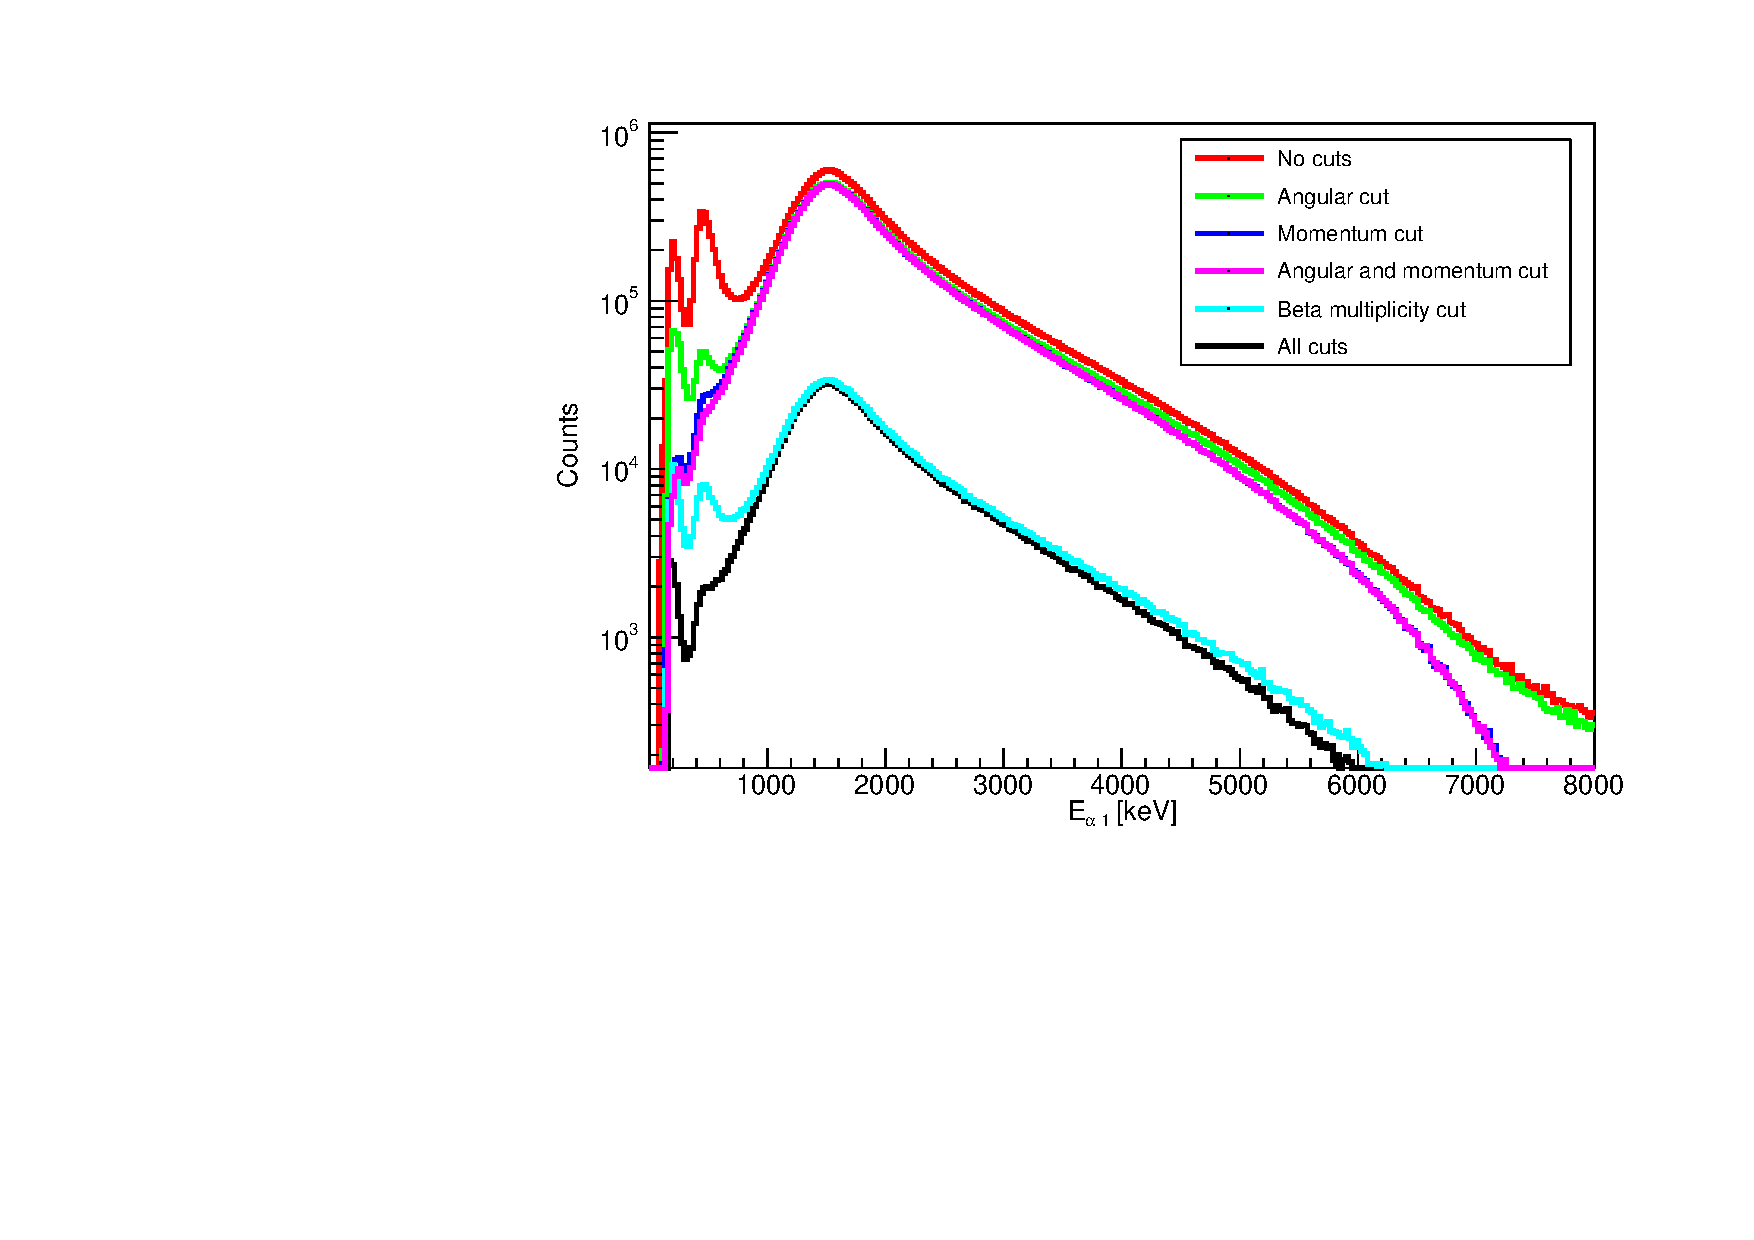
\includegraphics[width=.7\columnwidth]{../figures/cutCompare.pdf}
	\end{figure}
\end{frame}

\begin{frame}{\be\ energi spektrum}
	Falske \be\ identificeringer?
	\begin{figure}
		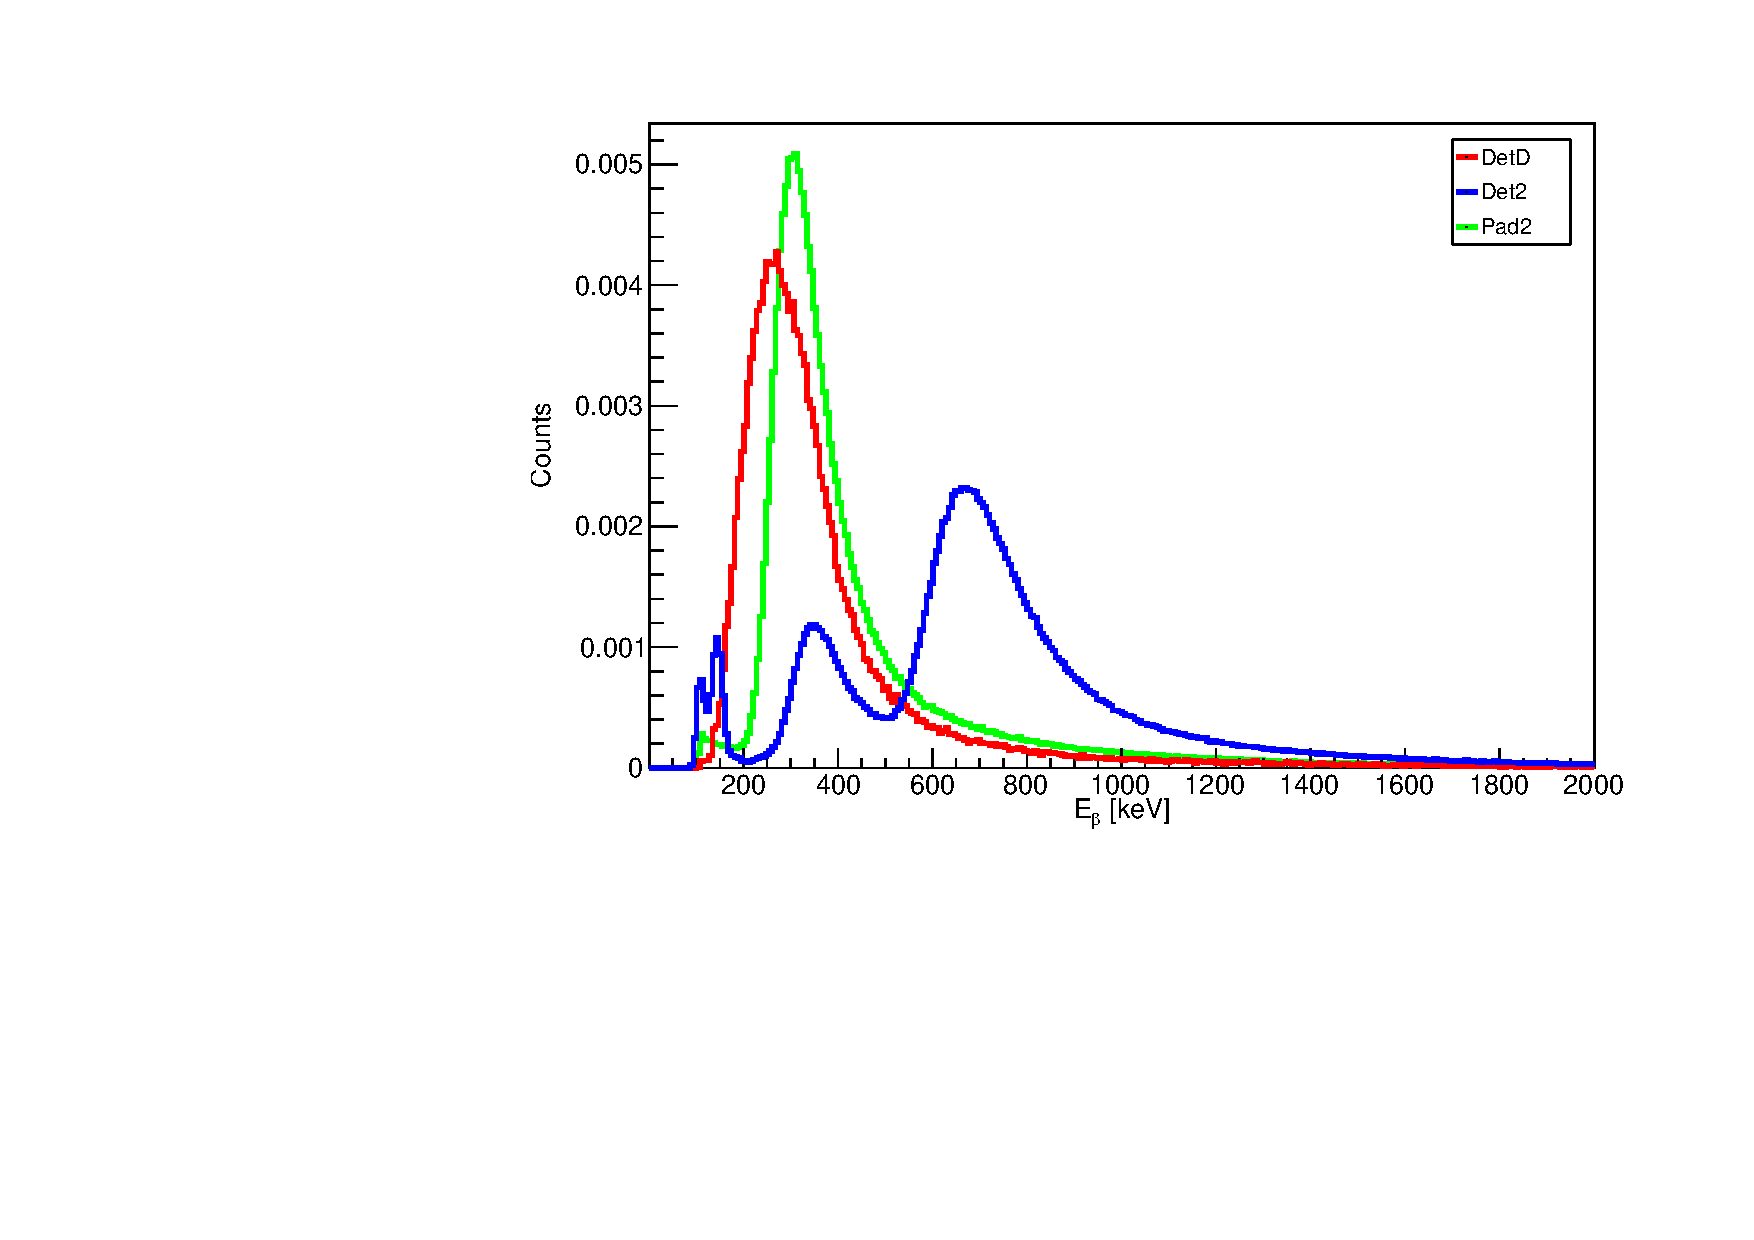
\includegraphics[width=.7\columnwidth]{../figures/betaSpec.pdf}
	\end{figure}
\end{frame}

\section{Data analyse}

\begin{frame}{Excitations spektrum for $^8$Be}
	Energi for summen af to \al-partikler\\
	Sammenligning med tidligere målinger \\
	God overensstemmelse for peak \\
	Lav niveau divagere meget fra hinanden
	\begin{figure}
		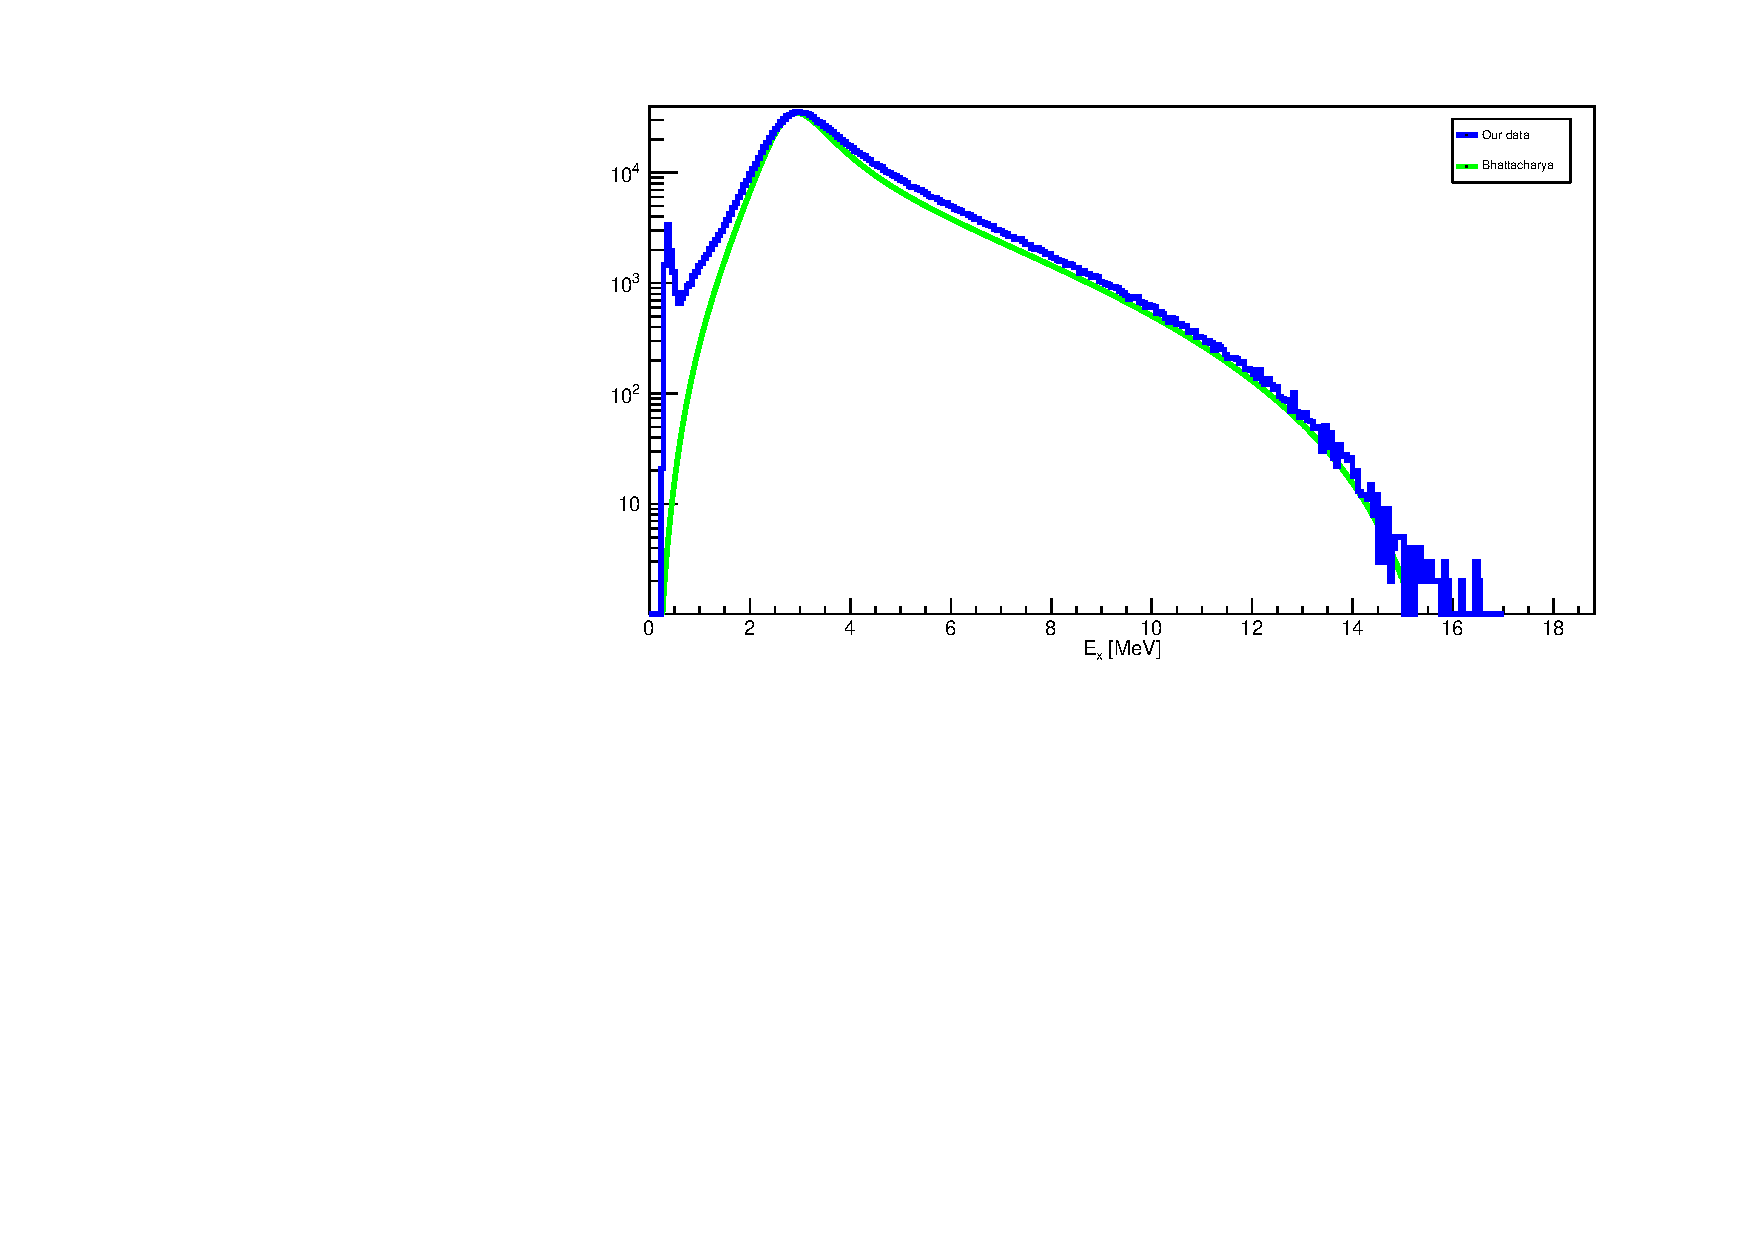
\includegraphics[width=.8\columnwidth]{../figures/bataraCompare.pdf}
	\end{figure}	
\end{frame}

\begin{frame}{Lepton rekyl - måske skip slide?}
	Forskel i energi mellem $\alpha_1$ og $\alpha_2$\\
	Indflydelse på $^8$Be peak\\
	Kan ikke undlades, som forslået af tidligere undersøgelser
	\begin{columns}
		\column[]{0.5\textwidth}\\
		\begin{figure}
			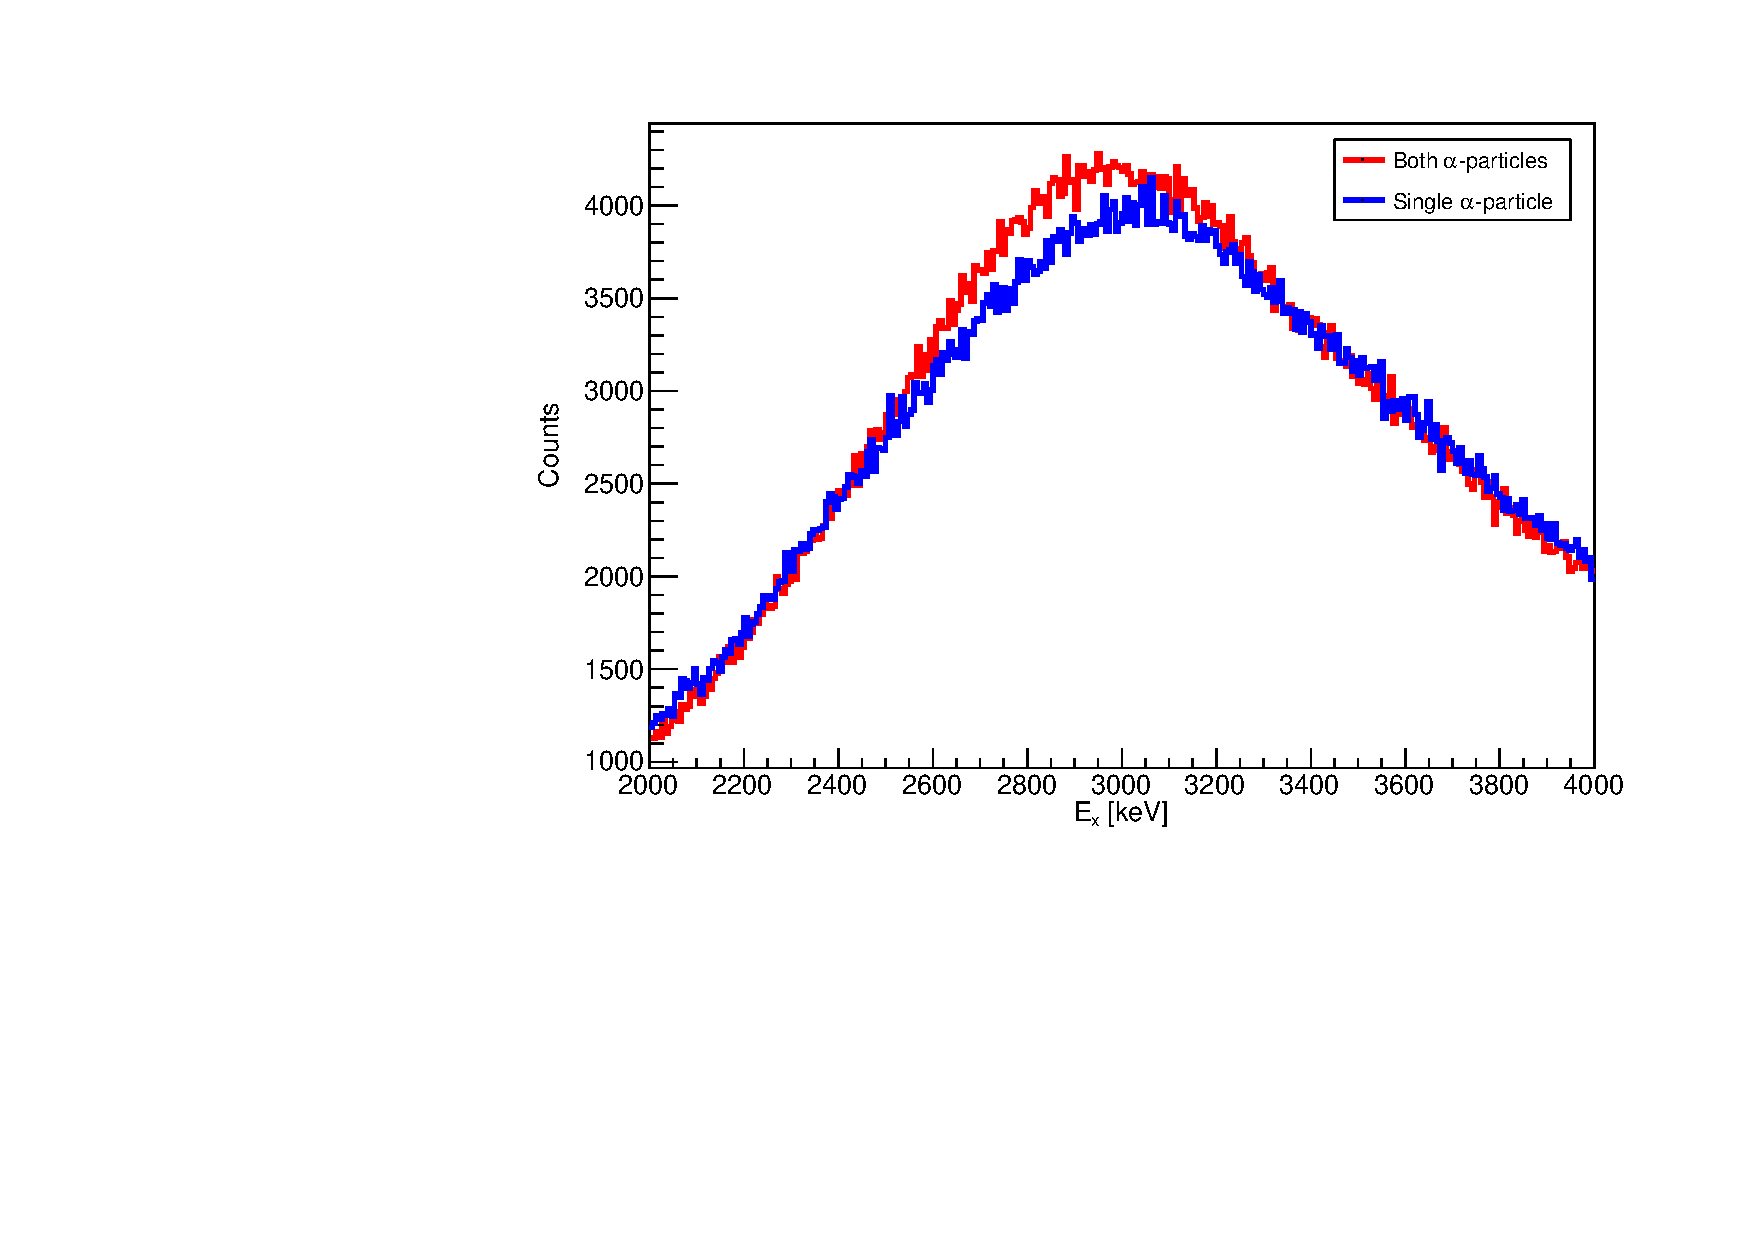
\includegraphics[width=\columnwidth]{../figures/recoil.pdf}
		\end{figure}
		\column[]{0.5\textwidth}\\
		\begin{figure}
			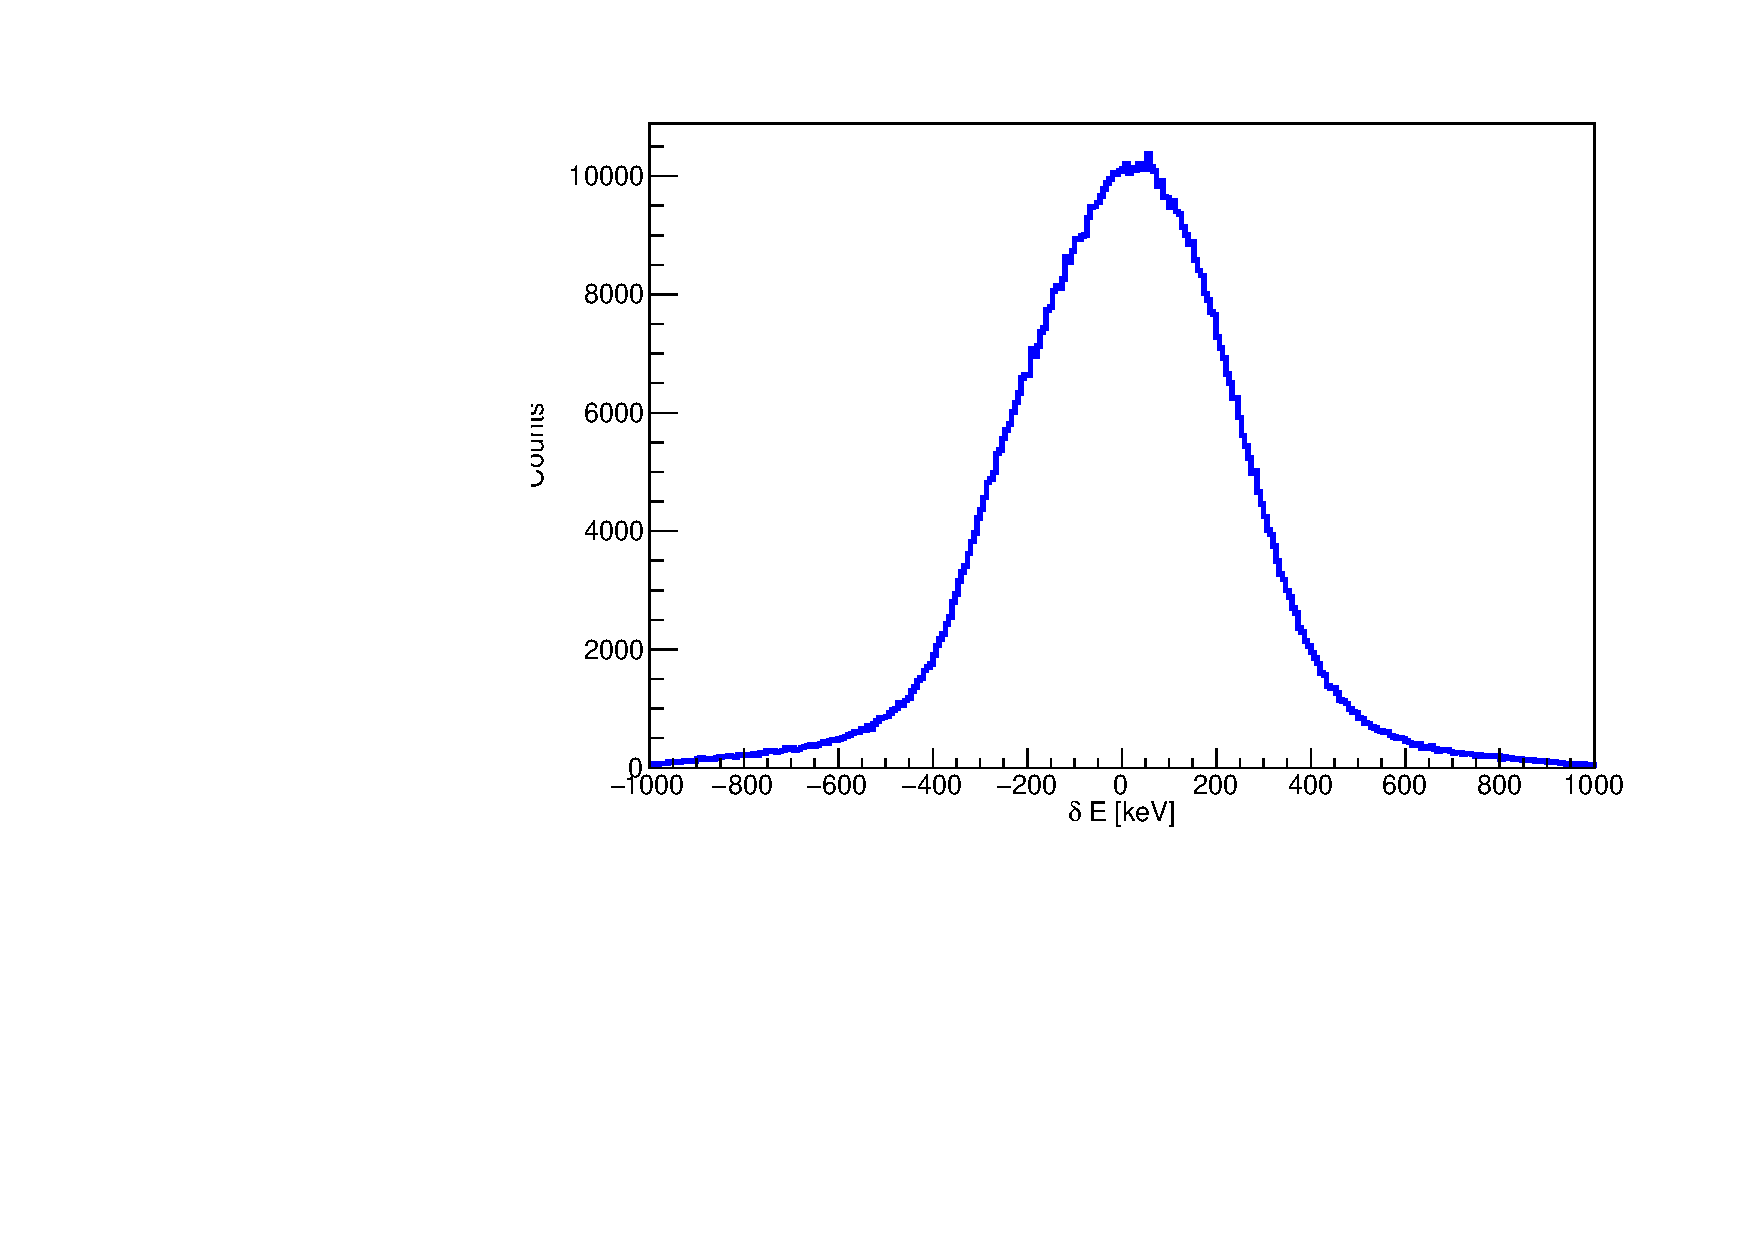
\includegraphics[width=\columnwidth]{../figures/recoilGauss.pdf}
		\end{figure}
	\end{columns}
\end{frame}

\begin{frame}{Vinkel korrelationer mellem \al\ og \be}
	Her er et plot lolleren
\end{frame}